%% Sections 1-3: introduction, framework and verification strategy
\section{Introduction}\label{sec:intro}

Minimum-weight design of steel moment frames with discrete catalogue sections is a mature
topic in structural optimisation. Genetic algorithms \citep{Camp1998,Pezeshk2000}, harmony
search \citep{Degertekin2008} and a large family of other metaheuristics \citep{SakaGeem2013}
have been used to select hot-rolled sections that satisfy code strength and serviceability
checks at least weight. Almost all of this work is \emph{deterministic}: the optimiser drives
the governing load-and-resistance-factor design (LRFD) checks to unity and treats the partial
factors of the code as a sufficient representation of uncertainty. The partial factors,
however, were calibrated for members and typical load ratios \citep{Ellingwood1980,Galambos1982};
they do not guarantee a uniform reliability for an optimised \emph{system}, whose members are
all deliberately pushed to their limits and whose governing constraints may be strength in one
member group and drift in another. Optimising a frame against code checks can therefore produce
designs whose actual reliability is both non-uniform and unknown.

Reliability-based design optimisation (RBDO) replaces the deterministic checks by explicit
constraints on failure probabilities \citep{Frangopol1985,Enevoldsen1994}. The methodological
literature on RBDO is extensive \citep{Valdebenito2010,Aoues2010}, but applications to code-type
steel frame design with discrete sections remain rare, mainly because (i) estimating small
system failure probabilities inside a population-based optimiser is expensive, (ii) the
uncertainty models of loads and resistances must be consistent with the calibration basis of
the design code for the comparison with deterministic design to be meaningful, and (iii) the
analysis models are seldom verified independently, so that it is difficult to separate genuine
economic benefits from modelling artefacts. Studies of the system reliability of steel frames
designed by advanced analysis \citep{Buonopane2006,Zhang2016} have shown that the reliability
of code-designed frames varies substantially between configurations, which suggests that an
explicit reliability constraint could redistribute material more rationally.

This paper addresses the research question: \emph{can uncertainty-aware optimisation produce
more economical steel frame designs while satisfying explicit reliability and serviceability
constraints?} To answer it we develop and openly release a reproducible framework built on the
open-source finite element library PyNite \citep{PyNite}. The contributions are:
\begin{enumerate}
\item a parameterised generator of planar steel moment frames with discrete W-shape design
variables, AISC~360-16 \citep{AISC360} member checks and the Direct Analysis Method with
$B_1$--$B_2$ second-order amplification;
\item an exact superposition surrogate that turns five linear PyNite analyses per design into a
vectorised Monte Carlo evaluation of the system ultimate limit state (ULS) and two
serviceability limit states (SLS) for $5\times10^4$--$10^6$ samples, combined with a sample
average approximation \citep{Kleywegt2002} that makes the reliability constraints
deterministic functions of the design;
\item single-objective constrained genetic algorithms for deterministic (DDO) and
reliability-based (RBDO) optimisation and an NSGA-II \citep{Deb2002} formulation that
quantifies the trade-off between steel mass and system reliability;
\item a three-level verification: closed-form benchmarks, an independent solver (OpenSeesPy
\citep{McKenna2010,Zhu2018}) for linear and P-$\Delta$ responses, and a Monte Carlo study
with full second-order re-analysis of every sample that removes the simplifying assumptions of
the surrogate; and
\item a parametric study over number of storeys, bay width and wind pressure that shows where
uncertainty-aware design saves material, where it costs material, and why.
\end{enumerate}

Section~\ref{sec:framework} presents the frame family, the design checks, the probabilistic
model and the optimisation formulations. Section~\ref{sec:verification} verifies the structural
and reliability models. Section~\ref{sec:results} compares deterministic and uncertainty-aware
designs, presents the cost--reliability trade-off and the parametric and sensitivity studies.
Limitations and conclusions follow in Sections~\ref{sec:discussion} and \ref{sec:conclusions}.

%% ---------------------------------------------------------------------------
\section{Framework}\label{sec:framework}

\subsection{Parameterised frame family}\label{sec:frames}

The framework generates regular planar moment frames with $n_s$ storeys and $n_b$ bays of
width $b$ (Fig.~\ref{fig:frame}). All beam--column connections are rigid and column bases are
fixed. The ground storey is 4.5~m high and the upper storeys 3.8~m. Frames are spaced at
7.5~m, which defines the tributary width of floor loads and wind pressure. Nominal floor loads
are $q_D = 4.0$~kPa (slab, finishes and services) and $q_L = 2.4$~kPa (office occupancy); the
roof carries 3.0~kPa dead and 1.0~kPa live load. Member self-weight is added to the dead load.
The nominal 50-year wind is represented by a net (windward plus leeward) pressure $p_w$,
converted to storey forces from the tributary storey heights and distributed equally to the
floor nodes, which mimics a rigid floor diaphragm.

Members are grouped by storey groups of two storeys (three for the nine-storey frame); every
group has three discrete design variables: the exterior column, the interior column and the
beam section. Columns are selected from 20 W14 shapes (W14$\times$48 to W14$\times$311) and
beams from 28 W16--W30 shapes. All sections are ASTM A992 ($F_y = 345$~MPa,
$E = 200$~GPa). Section properties were taken from the AISC Shapes Database
\citep{AISCShapes}; as a guard against transcription errors, each entry was checked against
the fillet-free three-plate idealisation of the section, giving ratios of tabulated to plate
values of 0.99--1.03 for $A$, $I_x$, $Z_x$ and $I_y$ in all cases. The catalogues are sorted by
area so that an index step is a monotonic change in mass. A constructability constraint
requires column areas not to increase with height.

The base frame has six storeys, three 8-m bays and $p_w=1.2$~kPa. The parametric family
varies one parameter at a time (Table~\ref{tab:frames}): $n_s\in\{3,6,9\}$,
$b\in\{6,8,10\}$~m and $p_w\in\{0.8,1.2,1.6\}$~kPa.

\begin{figure}[!htbp]
\centering
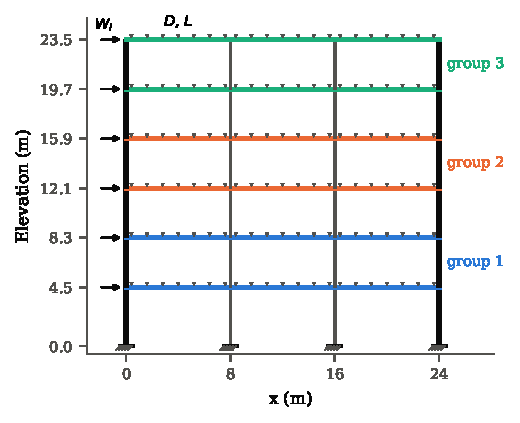
\includegraphics[width=0.55\textwidth]{figures/frame.pdf}
\caption{Base frame (six storeys, three 8-m bays). Thick lines: exterior columns; colours
indicate the three storey groups, each with an exterior-column, interior-column and beam
design variable. Gravity loads act on the beams; wind storey forces $W_i$ are applied at the
floor levels.}
\label{fig:frame}
\end{figure}

\begin{table}[!htbp]
\centering
\caption{Frames of the parametric study (one parameter varied at a time from the base frame).}
\label{tab:frames}
\small
\fittable{\begin{tabular}{lrrrrrr}
\toprule
Frame & Storeys & Bays & Bay (m) & $p_w$ (kPa) & Groups & Variables \\
\midrule
3 storeys & 3 & 3 & 8 & 1.2 & 2 & 6 \\
Base & 6 & 3 & 8 & 1.2 & 3 & 9 \\
9 storeys & 9 & 3 & 8 & 1.2 & 3 & 9 \\
Bay 6 m & 6 & 3 & 6 & 1.2 & 3 & 9 \\
Bay 10 m & 6 & 3 & 10 & 1.2 & 3 & 9 \\
$p_w$ = 0.8 kPa & 6 & 3 & 8 & 0.8 & 3 & 9 \\
$p_w$ = 1.6 kPa & 6 & 3 & 8 & 1.6 & 3 & 9 \\
\bottomrule
\end{tabular}}
\end{table}

\subsection{Structural analysis by superposition of PyNite unit cases}\label{sec:superposition}

For each candidate design $\mathbf{x}$, PyNite \citep{PyNite} solves five first-order linear
elastic load cases with nominal stiffness: dead load $D$ (including self-weight), live load
$L$, wind $W$, and two lateral cases $N_D$ and $N_L$ whose floor forces equal the dead and live
gravity load of each floor. Any realisation of the loading, with intensities
$(d,\ell,w)$ (multiples of the nominal $D$, $L$, $W$) and a global out-of-plumbness angle
$\theta$, then produces the first-order response
\begin{equation}
r = \underbrace{d\,r_D + \ell\,r_L}_{r_{nt}}
  + \underbrace{w\,r_W + \theta\,(d\,r_{N_D} + \ell\,r_{N_L})}_{r_{lt}},
\label{eq:superposition}
\end{equation}
split into the no-translation part $r_{nt}$ and the lateral-translation part $r_{lt}$
required by the approximate second-order analysis of AISC~360 Appendix~8. Because member
forces of a frame with uniformly scaled modulus $eE$ are independent of $e$ and displacements
scale with $1/e$, a global random modulus factor is also represented exactly. Responses
extracted per unit case are column end moments, axial and shear forces; beam moments at 11
stations along the span, axial and end shear forces; mid-span beam deflections relative to the
chord; and floor-average inter-storey drifts.

Second-order effects are introduced with the $B_1$--$B_2$ method. For storey $i$,
\begin{equation}
B_{2,i} = \left(1-\frac{P_{story,i}}{P_{e,story,i}}\right)^{-1},\qquad
P_{e,story,i} = R_M \,\tau\, e\,\frac{H_i h_i}{\Delta_{H,i}},
\label{eq:B2}
\end{equation}
where $P_{story,i}$ is the total gravity load carried by the storey, $H_i/\Delta_{H,i}$ the
first-order lateral stiffness obtained from the $W$ case, $h_i$ the storey height and
$R_M=0.85$. For columns, $B_1 = C_m/(1-P_r/P_{e1})\ge1$ with $C_m = 0.6-0.4M_1/M_2$
computed from the no-translation end moments and $P_{e1} = \pi^2\tau eEI/L^2$. Required
strengths are $M_r = B_1M_{nt} + B_2M_{lt}$ and $P_r = P_{nt}+B_2P_{lt}$; beams use the
larger $B_2$ of the two storeys they connect. A storey with $P_{story}\ge P_{e,story}$ is
unstable and is treated as failure. In deterministic design, the Direct Analysis Method (DAM)
\citep{AISC360,SurovekMaleck2004} is followed: stiffness is reduced by $\tau = 0.8$, notional
loads of $0.002Y_i$ are applied in gravity-only combinations and an additional $0.001Y_i$ in
all combinations so that $\tau_b=1$ may be used; effective length factors are then $K=1$.
In the reliability analysis the best-estimate stiffness ($\tau=1$) is used and the notional
loads are replaced by the random out-of-plumbness $\theta$.

\subsection{Member resistances and limit states}\label{sec:resistance}

Nominal resistances follow AISC~360-16: compression from Chapter~E3 with $K=1$, strong-axis
buckling over the storey height and weak-axis buckling between floors (columns) or between
secondary beams at third points (beams); flexure from F2 (lateral--torsional buckling, $C_b=1$)
and F3 (flange local buckling); shear from G2.1; and combined forces from the H1-1 interaction
equations. Beams carry axial forces that are small (the largest beam $P_r/P_c$ in the optimised
designs is reported below), so the slender-web reduction of beam compression capacity is not
modelled. For the deterministic design the LRFD resistance factors $\phi_c=\phi_b=\phi_t=0.9$
and $\phi_v=1.0$ or $0.9$ (G2.1) are applied to the five ASCE~7-05 \citep{ASCE705} strength
combinations $1.4D$, $1.2D+1.6L$, $1.2D+0.5L\pm1.6W$ and $0.9D\pm1.6W$ (roof live load is
treated as part of $L$). Serviceability requires inter-storey drift $\le h/400$ under
$D+0.5L+W$ and beam live-load deflection $\le$ span/360.

For each realisation the member utilisation $U_k$ is the larger of the H1-1 interaction ratio
and the shear ratio, both evaluated with nominal (unfactored) resistances that depend on the
random yield stress, modulus and fabrication factor of the member. Three limit-state functions
are defined:
\begin{align}
g_{ULS} &= 1 - \max_{s\in\{S_1,S_2\}}\max_k U_k^{(s)}, \label{eq:gULS}\\
g_{drift} &= 1 - \max_i \frac{\delta_i^{(S_2)}/h_i}{1/400}, \label{eq:gdrift}\\
g_{defl} &= 1 - \max_j \frac{\delta_{L,j}}{\ell_j/360}. \label{eq:gdefl}
\end{align}
The ULS is a series system over all members and over two load scenarios constructed with
Turkstra's rule \citep{TurkstraMadsen1980}: $S_1 = D + L_{50}$ (50-year maximum live load)
and $S_2 = D + L_{apt} + W_{50}$ (arbitrary-point-in-time live load with the 50-year maximum
wind); the out-of-plumbness acts in both. The drift SLS is evaluated in $S_2$ and the
deflection SLS under $L_{50}$. Note that $g_{ULS}$ measures the first attainment of a
code-format member limit state in a second-order elastic analysis; it is not a collapse
analysis and does not credit inelastic redistribution, consistent with the component-based
calibration of current codes.

\subsection{Probabilistic model}\label{sec:probmodel}

Table~\ref{tab:rv} lists the basic random variables. The load statistics are those of the
probability-based load criterion of \citet{Ellingwood1980} for dead load, 50-year live load and
50-year wind; the arbitrary-point-in-time live load follows a gamma distribution with mean
$0.24L_n$ and c.o.v.\ 0.60, and the fabrication (geometric) factor has c.o.v.\ 0.05 as in the
same study. The c.o.v.\ of yield stress (0.07) and modulus (0.03) and the lognormal model are
those of the JCSS Probabilistic Model Code \citep{JCSS2001}. The mean-to-nominal ratio of
$F_y$ (1.10) is an assumption of this study; its influence and that of the inter-member
correlation of $F_y$ (equicorrelation $\rho=0.5$ in log space between members of one frame) are
examined in the sensitivity study. The initial out-of-plumbness is normal with zero mean and
standard deviation 1/1000, so that the erection tolerance of 1/500 corresponds to two standard
deviations. Load intensities and $E$ are fully correlated over the frame; $F_y$ and the
fabrication factor are member-specific.

\begin{table}[!htbp]
\centering
\caption{Basic random variables (50-year reference period).}
\label{tab:rv}
\small
\fittable{\begin{tabular}{llcc}
\toprule
Variable & Distribution & Mean/nominal & CoV \\
\midrule
Dead load $D$ & Normal & 1.05 & 0.10 \\
50-yr max. live load $L_{50}$ & Gumbel & 1.00 & 0.25 \\
Arbitrary-point-in-time live load $L_{apt}$ & Gamma & 0.24 & 0.60 \\
50-yr max. wind load $W_{50}$ & Gumbel & 0.78 & 0.37 \\
Elastic modulus $E$ & Lognormal & 1.00 & 0.03 \\
Yield stress $F_y$ (per member) & Lognormal & 1.10 & 0.07 \\
Fabrication factor $F$ (per member) & Normal & 1.00 & 0.05 \\
Out-of-plumbness $\theta$ (rad) & Normal & 0 & s.d. 1/1000 \\
\bottomrule
\end{tabular}}
\end{table}

\subsection{Reliability estimation and sample average approximation}\label{sec:mc}

Failure probabilities are estimated by crude Monte Carlo simulation,
$\hat P_f = N^{-1}\sum_{n}\mathbb{1}[g(\mathbf{X}_n)\le0]$, with c.o.v.\
$\sqrt{(1-P_f)/(NP_f)}$, and reported as $\beta = -\Phi^{-1}(\hat P_f)$. Because the limit
states are evaluated by the superposition~\eqref{eq:superposition} and closed-form
resistances, the cost of a sample is a few vectorised arithmetic operations per member; a
design is evaluated with $5\times10^4$ samples in about one second on one CPU core, about
four times the cost of the five PyNite analyses.

Inside the optimiser the samples are drawn once and reused for every design (common random
numbers). This sample average approximation \citep{Kleywegt2002} makes $\hat\beta(\mathbf{x})$
a deterministic function of the design, so that the comparison of two designs is not corrupted
by sampling noise and the discrete search is well posed. To save time, a design is first
evaluated on the first $10^4$ samples and the remainder is computed only if the screening
estimate is not clearly infeasible (more than 0.4 below a target index). Every final design is
then re-verified with $N=10^6$ \emph{independent} samples, which provides an unbiased estimate
of its reliability and exposes any optimisation bias of the SAA. When no failure occurs in the
sample, $\hat P_f$ is replaced by $0.5/N$ and the reported $\beta$ is a lower bound.

\subsection{Optimisation formulations}\label{sec:optimisation}

The objective is the material cost, taken as proportional to the steel mass
$m(\mathbf{x}) = \rho_s\sum_k A_k(\mathbf{x})\ell_k$. Connection, fabrication and erection
costs are not modelled. Three formulations are compared:
\begin{align}
\text{DDO:}\quad &\min_{\mathbf{x}}\ m(\mathbf{x})\quad\text{s.t.}\quad
\max_{c,k}U^{LRFD}_{c,k}\le1,\quad \frac{\delta}{h}\le\frac{1}{400},\quad \delta_L\le\frac{\ell}{360},\\
\text{RBDO:}\quad &\min_{\mathbf{x}}\ m(\mathbf{x})\quad\text{s.t.}\quad
\beta_{ULS}\ge\beta_T,\quad \beta_{drift}\ge\beta_{SLS},\quad \beta_{defl}\ge\beta_{SLS},\\
\text{MO:}\quad &\min_{\mathbf{x}}\ \bigl(m(\mathbf{x}),\,-\beta_{ULS}(\mathbf{x})\bigr)\quad\text{s.t.}\quad
\beta_{drift},\beta_{defl}\ge\beta_{SLS},\quad \beta_{ULS}\ge1,
\end{align}
all subject to column areas that do not increase with height.
The baseline targets are $\beta_T = 3.0$ for the system ULS, the value adopted by
\citet{Ellingwood1980} for gravity load combinations in the calibration of the LRFD load
factors (a lower value was accepted for combinations with wind), and $\beta_{SLS}=1.5$ (50 years), the value given by EN~1990
\citep{EN1990} for irreversible serviceability states. Because both targets are
choices of the owner or code writer, results are also given for other targets.

DDO and RBDO are solved with the same elitist genetic algorithm (population 40, at most 60
generations, binary tournament with Deb's feasibility rules \citep{Deb2000}, uniform crossover
with probability 0.9, per-gene mutation probability $1.5/n_v$ of which 70\% are steps of
$\pm1$--3 catalogue positions and 30\% random resets, $(\mu+\lambda)$ replacement, and
termination after 15 generations without improvement). The best GA design is polished by a
discrete local search that accepts the first feasible lighter neighbour among single
down-sizing moves and down/up-sizing swaps of two variables, repeated until no improvement is
found. The bi-objective problem is solved with NSGA-II \citep{Deb2002} with constrained
domination (population 48, 60 generations); all feasible designs visited are archived and the
non-dominated archive is reported. The SAA samples, the GA operators and the verification
samples are all seeded, so every number in this paper is reproducible from the released code.

%% ---------------------------------------------------------------------------
\section{Verification of the structural and reliability models}\label{sec:verification}
